% Important: If latex complains about unicode characters,
% please use "\usepackage[utf8x]{inputenc}" in your preamble
% You can change the size of the picture by putting it into the construct:
% 1) \resizebox{10cm}{!}{"below picture"} to scale horizontally to 10 cm
% 2) \resizebox{!}{15cm}{"below picture"} to scale vertically to 15 cm
% 3) \resizebox{10cm}{15cm}{"below picture"} a combination of above two
% It is not recomended to use the scale option of the tikzpicture environment.
\resizebox{6cm}{!}{
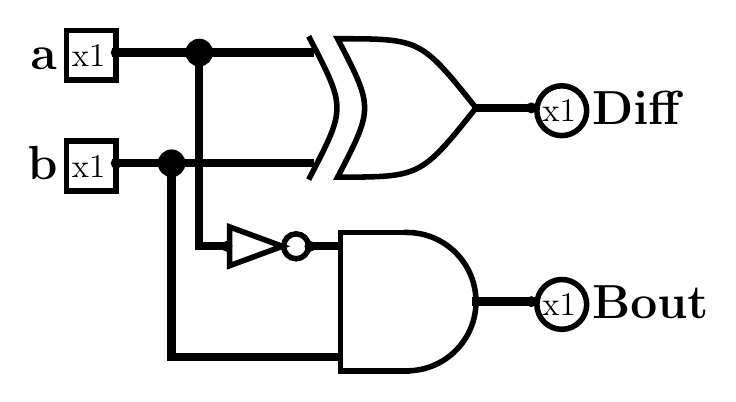
\begin{tikzpicture}[x=1pt,y=-1pt,line cap=rect]
\def\logisimfontA#1{\fontfamily{cmr}{#1}} % Replaced by logisim, original font was "SansSerif"
\definecolor{custcol_0_0_0}{RGB}{0, 0, 0}
\definecolor{custcol_ff_ff_ff}{RGB}{255, 255, 255}
\draw [line width=3.0pt, custcol_0_0_0 ]  (37.0,15.0) -- (67.0,15.0) -- (67.0,85.0) -- (77.0,85.0) ;
\draw [line width=3.0pt, custcol_0_0_0 ]  (107.0,85.0) -- (117.0,85.0) ;
\draw [line width=3.0pt, custcol_0_0_0 ]  (167.0,35.0) -- (187.0,35.0) ;
\draw [line width=3.0pt, custcol_0_0_0 ]  (167.0,105.0) -- (187.0,105.0) ;
\draw [line width=3.0pt, custcol_0_0_0 ]  (37.0,55.0) -- (57.0,55.0) ;
\fill [line width=3.0pt, custcol_0_0_0]  (57.0,55.0) ellipse (5.0 and 5.0 );
\fill [line width=3.0pt, custcol_0_0_0]  (67.0,15.0) ellipse (5.0 and 5.0 );
\draw [line width=2.0pt, custcol_0_0_0 ]  (19.0,7.0) -- (36.0,7.0) ;
\draw [line width=2.0pt, custcol_0_0_0 ]  (37.0,7.0) -- (37.0,24.0) ;
\draw [line width=2.0pt, custcol_0_0_0 ]  (37.0,25.0) -- (20.0,25.0) ;
\draw [line width=2.0pt, custcol_0_0_0 ]  (19.0,25.0) -- (19.0,8.0) ;
\logisimfontA{\fontsize{12pt}{12pt}\selectfont\node[inner sep=0, outer sep=0, custcol_0_0_0, anchor=base west] at  (21.0,20.0)  {x1};}
\logisimfontA{\fontsize{16pt}{16pt}\fontseries{bx}\selectfont\node[inner sep=0, outer sep=0, custcol_0_0_0, anchor=base west] at  (6.0,21.0)  {a};}
\fill [line width=2.0pt, custcol_0_0_0]  (37.0,15.0) ellipse (2.0 and 2.0 );
\draw [line width=2.0pt, custcol_0_0_0 ]  (19.0,47.0) -- (36.0,47.0) ;
\draw [line width=2.0pt, custcol_0_0_0 ]  (37.0,47.0) -- (37.0,64.0) ;
\draw [line width=2.0pt, custcol_0_0_0 ]  (37.0,65.0) -- (20.0,65.0) ;
\draw [line width=2.0pt, custcol_0_0_0 ]  (19.0,65.0) -- (19.0,48.0) ;
\logisimfontA{\fontsize{12pt}{12pt}\selectfont\node[inner sep=0, outer sep=0, custcol_0_0_0, anchor=base west] at  (21.0,60.0)  {x1};}
\logisimfontA{\fontsize{16pt}{16pt}\fontseries{bx}\selectfont\node[inner sep=0, outer sep=0, custcol_0_0_0, anchor=base west] at  (5.0,61.0)  {b};}
\fill [line width=2.0pt, custcol_0_0_0]  (37.0,55.0) ellipse (2.0 and 2.0 );
\draw [line width=3.0pt, custcol_0_0_0 ]  (67.0,15.0) -- (107.0,15.0) -- (107.0,15.0) ;
\draw [line width=3.0pt, custcol_0_0_0 ]  (117.0,125.0) -- (57.0,125.0) -- (57.0,55.0) -- (107.0,55.0) -- (107.0,55.0) ;
\draw [line width=2.0pt, custcol_0_0_0 ]  (167.0,35.0) .. controls  (147.0,10.0)  ..  (117.0,10.0) .. controls  (130.0,35.0)  ..  (117.0,60.0) .. controls  (147.0,60.0)  ..  (167.0,35.0) -- cycle ;
\draw [line width=2.0pt, custcol_0_0_0 ]  (107.0,10.0) .. controls  (120.0,35.0)  ..  (107.0,60.0) ;
\draw [line width=2.0pt, custcol_0_0_0]  (198.0,36.0) ellipse (9.0 and 9.0 );
\logisimfontA{\fontsize{12pt}{12pt}\selectfont\node[inner sep=0, outer sep=0, custcol_0_0_0, anchor=base west] at  (191.0,40.0)  {x1};}
\logisimfontA{\fontsize{16pt}{16pt}\fontseries{bx}\selectfont\node[inner sep=0, outer sep=0, custcol_0_0_0, anchor=base west] at  (209.0,41.0)  {Diff};}
\fill [line width=2.0pt, custcol_0_0_0]  (187.0,35.0) ellipse (2.0 and 2.0 );
\draw [line width=2.0pt, custcol_0_0_0 ]  (97.0,85.0) -- (78.0,78.0) -- (78.0,92.0) -- cycle;
\draw [line width=2.0pt, custcol_0_0_0]  (102.0,85.0) ellipse (4.5 and 4.5 );
\fill [line width=2.0pt, custcol_0_0_0]  (107.0,85.0) ellipse (2.0 and 2.0 );
\fill [line width=2.0pt, custcol_0_0_0]  (77.0,85.0) ellipse (2.0 and 2.0 );
\draw [line width=2.0pt, custcol_0_0_0]  (198.0,106.0) ellipse (9.0 and 9.0 );
\logisimfontA{\fontsize{12pt}{12pt}\selectfont\node[inner sep=0, outer sep=0, custcol_0_0_0, anchor=base west] at  (191.0,110.0)  {x1};}
\logisimfontA{\fontsize{16pt}{16pt}\fontseries{bx}\selectfont\node[inner sep=0, outer sep=0, custcol_0_0_0, anchor=base west] at  (209.0,111.0)  {Bout};}
\fill [line width=2.0pt, custcol_0_0_0]  (187.0,105.0) ellipse (2.0 and 2.0 );
\draw [line width=2.0pt, custcol_0_0_0] (142.0,130.0) arc (90.0:-90.0:25.0 and 25.0 );
\draw [line width=2.0pt, custcol_0_0_0 ]  (142.0,80.0) -- (118.0,80.0) -- (118.0,130.0) -- (142.0,130.0) ;
\end{tikzpicture}
}
